\documentclass[12pt, twoside]{article}
\usepackage[letterpaper, margin=1in, head=30pt, headsep=0.1in]{geometry}
\usepackage[english]{babel}
\usepackage[utf8]{inputenc}
\usepackage{amsmath}
\usepackage{amsfonts}
\usepackage{amssymb}
\usepackage{tikz}
\usetikzlibrary{quotes, angles}

\usepackage{graphicx}
\usepackage{enumitem}
\usepackage{multicol}

%\usepackage{pgfplots}
%\pgfplotsset{width=10cm,compat=1.9}
%\usepgfplotslibrary{statistics}
%\usepackage{pgfplotstable}
%\usepackage{tkz-fct}
%\usepackage{venndiagram}

\usepackage{fancyhdr}
\pagestyle{fancy}
\fancyhf{}
\renewcommand{\headrulewidth}{0pt} % disable the underline of the header
\raggedbottom
\newif\ifmeta
\metatrue %print standards and topics tags

\title{Math AI Worksheet Generator and Formative Assessment System}
\author{Chris Huson}
\date{October 2020}

%\fancyhead[RE]{\thepage}
%\fancyhead[RO]{\thepage \\ Name: \hspace{3cm}}
%\fancyhead[L]{BECA / Dr. Huson / 10th Grade Geometry\\* 7 June 2019}
%
%\begin{document}
%\subsubsection*{13.7 Homework: Cross sections, distance applications}
%\fancyhead[L]{BECA / Dr. Huson / Geometry 03-Volume+angle-bisectors\\* pset ID: 34}

\begin{document}

\subsubsection*{Unit 1 Re-Quiz: Spicy problems}
\begin{enumerate}

\item Given point $A(-1)$ as shown below. Locate point, $B > 0$, on the number line such that ${AB}=3 \frac{1}{2}$. \\[1.5cm]
    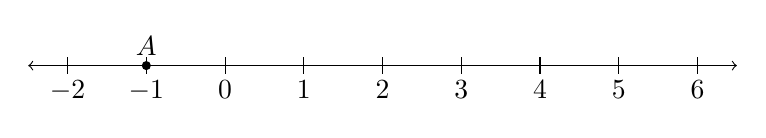
\begin{tikzpicture}
      \draw [<->] (-2.5,0)--(6.5,0);
      %\draw [-, thick] (1,0)--(4.5,0);
      \foreach \x in {-2,...,6} %2 leading for diff!=1
        \draw[shift={(\x,0)},color=black] (0pt,-3pt) -- (0pt,3pt) node[below=5pt]  {$\x$};
        \draw [fill] (-1,0) circle [radius=0.05] node[above] {$A$};
        %\draw [fill] (4.5,0) circle [radius=0.05] node[above] {$N$};
    \end{tikzpicture}
    \begin{enumerate}
      \item Mark and label $B$.
      \item State the value of $B$, writing an equation to support your work.
    \end{enumerate} \vspace{3cm}  

\newpage
\item Given $M$ is the midpoint of $\overline{AB}$, $AM=5x+11$, $MB=x+21$.
  \begin{enumerate}
    \item Mark the diagram with the values and tick marks
    \item Write an equation and solve for $x$
    \item Check your result
  \end{enumerate} \vspace{1cm}
    \begin{center}
      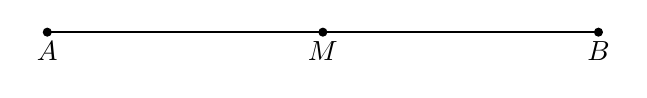
\begin{tikzpicture}
        \draw [fill] (0,0) circle [radius=0.05] node[below]{$A$};
        \draw [-, thick] (0,0)--(7,0);
        \draw [fill] (3.5,0) circle [radius=0.05] node[below]{$M$};
        \draw [fill] (7,0) circle [radius=0.05] node[below]{$B$};
        %\node at (1.7,0.5) [above]{$x+2$};
        %\node at (5.2,0.5) [above]{$11$};
        %\draw [<->, dashed] (0,-1)--(7,-1);
        %\node at (3.5,-1) [below]{$20$};
      \end{tikzpicture}
    \end{center} \vspace{4cm}

\newpage
\item Given $S(-1.3)$ and $T(3.3)$, as shown on the number line. \\[0.25cm]
      Mark and label the midpoint $M$ that bisects $\overline{ST}$. \\[0.5cm]
        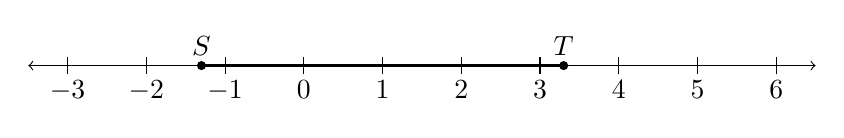
\begin{tikzpicture}
          \draw [<->] (-3.5,0)--(6.5,0);
          \draw [-, thick] (-1.3,0)--(3.3,0);
          \foreach \x in {-3,...,6} %2 leading for diff!=1
            \draw[shift={(\x,0)},color=black] (0pt,-3pt) -- (0pt,3pt) node[below=5pt]  {$\x$};
            \draw [fill] (-1.3,0) circle [radius=0.05] node[above] {$S$};
            \draw [fill] (3.3,0) circle [radius=0.05] node[above] {$T$};
        \end{tikzpicture} \vspace{4cm}  
    
\newpage
\item The perimeter of the isosceles $\triangle FGH$ is 35 with $\overline{FH} \cong \overline{GH}$. If $FG=x+5$ and $FH=13 \frac{1}{2}$, find $x$.\\[0.25cm]
    Show your work with an equation for full credit.\\[0.5cm]
      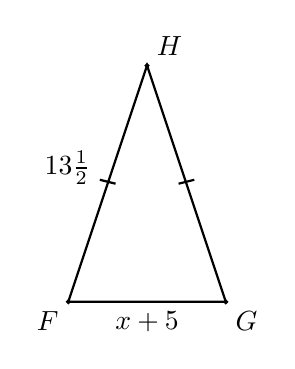
\begin{tikzpicture}[scale=0.5]
        \draw [thick](0,0)--(4,0)--(2,6)--(0,0);
        \draw [fill] (0,0) circle [radius=0.05] node[below left]{$F$};
        \draw [fill] (4,0) circle [radius=0.05] node[below right]{$G$};
        \draw [fill] (2,6) circle [radius=0.05] node[above right]{$H$};
        \draw [thick] (0.8,3.1)--(1.2,3); %tick mark
        \draw [thick] (2.8,3)--(3.2,3.1); %tick mark
        \node at (2,0) [below]{$x+5$};
        \node at (0.8,3.4) [left]{$13 \frac{1}{2}$};
      \end{tikzpicture} \vspace{1cm}

\newpage
\item Given $\overline{PQR}$, $PQ=2x+11$, $QR=x+1$, $PR=x+26$. Find ${x}$.
  \begin{center}
      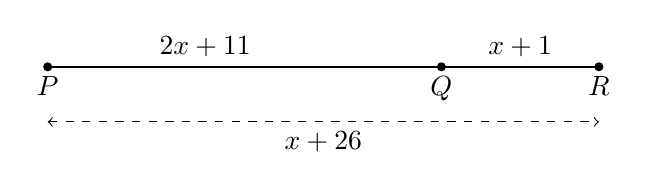
\begin{tikzpicture}
      \draw [-, thick] (0,0)--(7,0);
      \draw [fill] (0,0) circle [radius=0.05] node[below]{$P$};
      \draw [fill] (5,0) circle [radius=0.05] node[below]{$Q$};
      \draw [fill] (7,0) circle [radius=0.05] node[below]{$R$};
      \node at (2,0) [above]{$2x+11$};
      \node at (6,0) [above]{$x+1$};
      \draw [<->, dashed] (0,-0.7)--(7,-0.7);
      \node at (3.5,-0.7) [below]{$x+26$};
    \end{tikzpicture}
  \end{center}
  \begin{enumerate}
      \item Write down an equation to represent the situation. \vspace{0.5cm}
      \item Solve for $x$. \vspace{1.5cm}
      \item Check your answer. \vspace{2cm}
    \end{enumerate}

\newpage
\item Given the points $S$ and $T$ trisect the line segment $\overline{RU}$, as shown below. If $RT=7$, find $RU$.\\[1cm]
    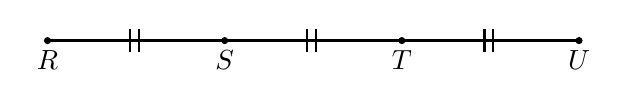
\begin{tikzpicture}[scale=0.75]
     \draw [-, thick] (0,0)--(9,0);
     \draw [fill] (0,0) circle [radius=0.05] node[below]{$R$};
     \draw [fill] (3,0) circle [radius=0.05] node[below]{$S$};
     \draw [fill] (6,0) circle [radius=0.05] node[below]{$T$};
     \draw [fill] (9,0) circle [radius=0.05] node[below]{$U$};
     %\node at (1.6,0.3) [above]{$x$};
     %\node at (4.6,0.3) [above]{$x$};
     %\node at (7.6,0.3) [above]{$x$};
     \draw [-, thick] (1.4,-0.2)--(1.4,0.2);
     \draw [-, thick] (1.55,-0.2)--(1.55,0.2);
     \draw [-, thick] (4.4,-0.2)--(4.4,0.2);
     \draw [-, thick] (4.55,-0.2)--(4.55,0.2);
     \draw [-, thick] (7.4,-0.2)--(7.4,0.2);
     \draw [-, thick] (7.55,-0.2)--(7.55,0.2);
     %\draw [<->, dashed] (0,-1.3)--(9,-1.3);
     %\node at (4.5,-1.3) [below]{$15$};
   \end{tikzpicture} \vspace{3cm}

\newpage
\item Given $A(-2.1)$ and $M(1.8)$, as shown on the number line. The point $B$ is such that $M$ bisects $\overline{AB}$. \\[0.25cm] 
Find the value of $B$. Mark and label it on the number line.\\[0.5cm]
        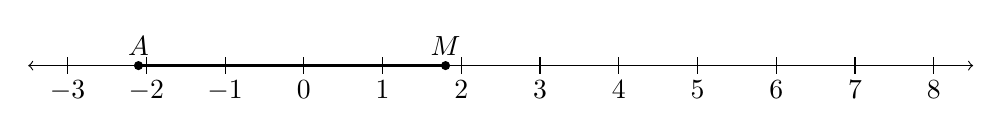
\begin{tikzpicture}
          \draw [<->] (-3.5,0)--(8.5,0);
          \draw [-, thick] (-2.1,0)--(1.8,0);
          \foreach \x in {-3,...,8} %2 leading for diff!=1
            \draw[shift={(\x,0)},color=black] (0pt,-3pt) -- (0pt,3pt) node[below=5pt]  {$\x$};
            \draw [fill] (-2.1,0) circle [radius=0.05] node[above] {$A$};
            \draw [fill] (1.8,0) circle [radius=0.05] node[above] {$M$};
        \end{tikzpicture} \vspace{4cm}  

\newpage
\item The point $Q$ lies on $\overline{AB}$ three quarters of the way from $A$ to $B$. Given $AB=28$.
    \begin{enumerate}
      \item Mark and label the approximate location of $Q$.
      \item Find ${AQ}$. State an equation for full credit.
    \end{enumerate} \vspace{1cm} 
    \begin{center}
      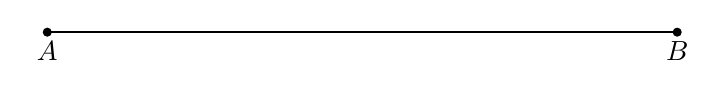
\begin{tikzpicture}
        \draw [-, thick] (0,0)--(8,0);
        \draw [fill] (0,0) circle [radius=0.05] node[below]{$A$};
        \draw [fill] (8,0) circle [radius=0.05] node[below]{$B$};
      \end{tikzpicture} 
    \end{center} \vspace{3cm} 

\end{enumerate}
\end{document}